
\subsubsection{Resistivity}
Copper resistivity depends on temperature and RRR:
\begin{equation}
    \rho_\text{N}(T, \text{RRR}) = \rho_\text{0}+\rho_\text{i}+\rho_\text{i0},
\end{equation}
\\
where:
\begin{equation}
    \rho_\text{0} = \frac{1.5553\cdot10^{-8}}{\text{RRR}}
\end{equation}

\begin{equation}
    \rho_\text{i} = \frac{\text{P}_\text{1}}{1+\text{P}_\text{1}  \text{P}_\text{3}  T^{\text{P}_\text{2} - \text{P}_\text{4}}  \exp{[-(\frac{\text{P}_\text{5}}{T}}^{\text{P}_\text{6}})]}
\end{equation}

\begin{equation}
    \rho_\text{i0} = \text{P}_\text{7} \frac{\rho_\text{i} \rho_\text{0}}{\rho_\text{i} + \rho_\text{0}}
\end{equation}
\\
In order to apply the resistivity dependence on magnetic field strength, the following formula are applied with fit parameters presented in Table \ref{table:nist_resistivity_parameters}:
\begin{equation}
    \rho_\text{N}(T, B, \text{RRR}) = \rho_\text{N}(T, \text{RRR}) \cdot (1 + 10^{a(x)}),  
\end{equation}
\\
where:
\begin{equation}
    a(x) = \sum_{n=0}^{N} a_\text{n}(\log_\text{10}x)^{n}
\end{equation}

\begin{equation}
    x \approx \frac{1.553 \cdot 10^{-8}}{\rho_\text{N}(T, \text{RRR})} \cdot B
\end{equation}

\begin{table}[h!]
    \caption{Fit parameters for NIST copper electrical resistivity} 
    \vspace{-1.em} 
    \fontsize{10}{10}
    \selectfont 
    \renewcommand{\arraystretch}{1.5}
    \begin{center}
    \begin{tabular}{ ccccccc }  
    \hline
    $\text{P}_1$ & $\text{P}_2$ & $\text{P}_3$ & $\text{P}_4$ & $\text{P}_5$ & $\text{P}_6$ & $\text{P}_7$ \\
    \hline
    $1.171\cdot10^{-17}$ & 4.49 & $3.841\cdot10^{10}$ & 1.14 & 50 & 6.428 & 0.4531 \\
    \hline 
    \end{tabular}
    \\
    \begin{tabular}{ ccccc }  
    $\text{a}_0$ & $\text{a}_1$ & $\text{a}_2$ & $\text{a}_3$ & $\text{a}_4$ \\
    \hline
    -2.662 & 0.3168 & 0.6229 & -0.1839 & 0.001827 \\
    \hline
    \end{tabular}
    \end{center}  
     \label{table:nist_resistivity_parameters} 
 \end{table}

Fig. \ref{fig:cu_resistivity_plot} shows copper resistivity for low and high value of RRR. In general, it rises with temperature, decrease of RRR and increase of magnetic field strength.

\begin{figure}
\centering
\begin{tikzpicture}
\begin{axis}[
  no markers,
  legend style={at={(1,0)},anchor=south east},
  grid style={dashed,gray!30},
  width=0.85\linewidth, 
  height = 6cm,
  xlabel={$t$},
  ylabel={$\rho_{Cu}$},
  xlabel style={below right},
  ylabel style={above left},
  xmin=0.0,
  ymin=0.0,
  xmax=100.0
  ]
  
  \addplot table[x=Time,y=B_0_0_RRR_100,col sep=comma] {figures/material_properties/Cu_Rho_B_Depenedence.csv}; 
  \addplot table[x=Time,y=B_3_0_RRR_100,col sep=comma] {figures/material_properties/Cu_Rho_B_Depenedence.csv}; 
  \addplot table[x=Time,y=B_0_0_RRR_200,col sep=comma] {figures/material_properties/Cu_Rho_B_Depenedence.csv}; 
  \addplot table[x=Time,y=B_3_0_RRR_200,col sep=comma] {figures/material_properties/Cu_Rho_B_Depenedence.csv}; 
  
  \legend{$B(\text{RRR}=100)=0~\text{T}$,
  $B(\text{RRR}=100)=3~\text{T}$,
  $B(\text{RRR}=200)=0~\text{T}$,
  $B(\text{RRR}=200)=3~\text{T}$}

\end{axis}
\end{tikzpicture}
\caption{Copper resistivity temperature dependence for varying magnetic field and RRR}
    \label{fig:cu_resistivity_plot}
\end{figure}

%  thermal conductivity
\subsubsection{Thermal Conductivity}
Copper thermal conductivity depends on temperature and RRR:
\begin{equation}
    k_\text{N}(T, \text{RRR}) = \frac{1}{\text{W}_\text{0} + \text{W}_\text{i} + \text{W}_\text{i0}}, 
\end{equation}
\\ 
where:
\begin{equation}
    \text{W}_\text{0} = \frac{\beta}{T}
\end{equation}

\begin{equation}
    \text{W}_\text{i} = \frac{\text{P}_\text{1} T^{\text{P}_\text{2}}}{1+\text{P}_\text{1}  \text{P}_\text{3}  T^{\text{P}_\text{2} + \text{P}_\text{4}}  \exp{[-(\frac{\text{P}_\text{5}}{T}}^{\text{P}_\text{6}})]}
\end{equation}

\begin{equation}
    \text{W}_\text{i0} = \text{P}_\text{7} \frac{\text{W}_\text{i} \text{W}_\text{0}}{\text{W}_\text{i} + \text{W}_\text{0}}
\end{equation}
\\
with fit parameters presented in Table \ref{table:nist_cu_k_parameters}.

\begin{table}[h!]
    \caption{Fit parameters for NIST copper thermal conductivity} 
    \vspace{-1.em} 
    \fontsize{10}{10}
    \selectfont 
    \renewcommand{\arraystretch}{1.5}
    \begin{center}
    \begin{tabular}{ cc }  
    $\beta$ & $\beta_\text{r}$ \\
    \hline
    $0.634/\text{RRR}$ & $\beta/0.0003$ \\
    \hline
    \end{tabular}
    
    \begin{tabular}{ ccccccc }  
    $\text{P}_1$ & $\text{P}_2$ & $\text{P}_3$ & $\text{P}_4$ & $\text{P}_5$ & $\text{P}_6$ & $\text{P}_7$ \\
    \hline
    $1.754\cdot10^{-8}$ & 2.763 & 1102 & -0.165 & 70 & 1.756 & $0.838/\beta_\text{r}^{0.1661}$ \\
    \hline 
    \end{tabular}
    \end{center}  
     \label{table:nist_cu_k_parameters} 
 \end{table}
 
 In order to include the magnetic induction dependence in the function of thermal conductivity, one can apply: 
\begin{equation}
    k_\text{N}(T, B, \text{RRR}) = \frac{\rho\text{N}(T, B=0, \text{RRR})}{\rho\text{N}(T, B=0, \text{RRR})} \cdot k_\text{N}(T, \text{RRR})
\end{equation}

As presented in Fig. \ref{fig:cu_k_plot}, thermal conductivity decreases with increase of magnetic field strength and when a cable is characterised by lower RRR. One can also notice that the peak value of thermal conductivity occurs at lower temperatures when RRR is high. 
 
\begin{figure}[h!]
    \centering
    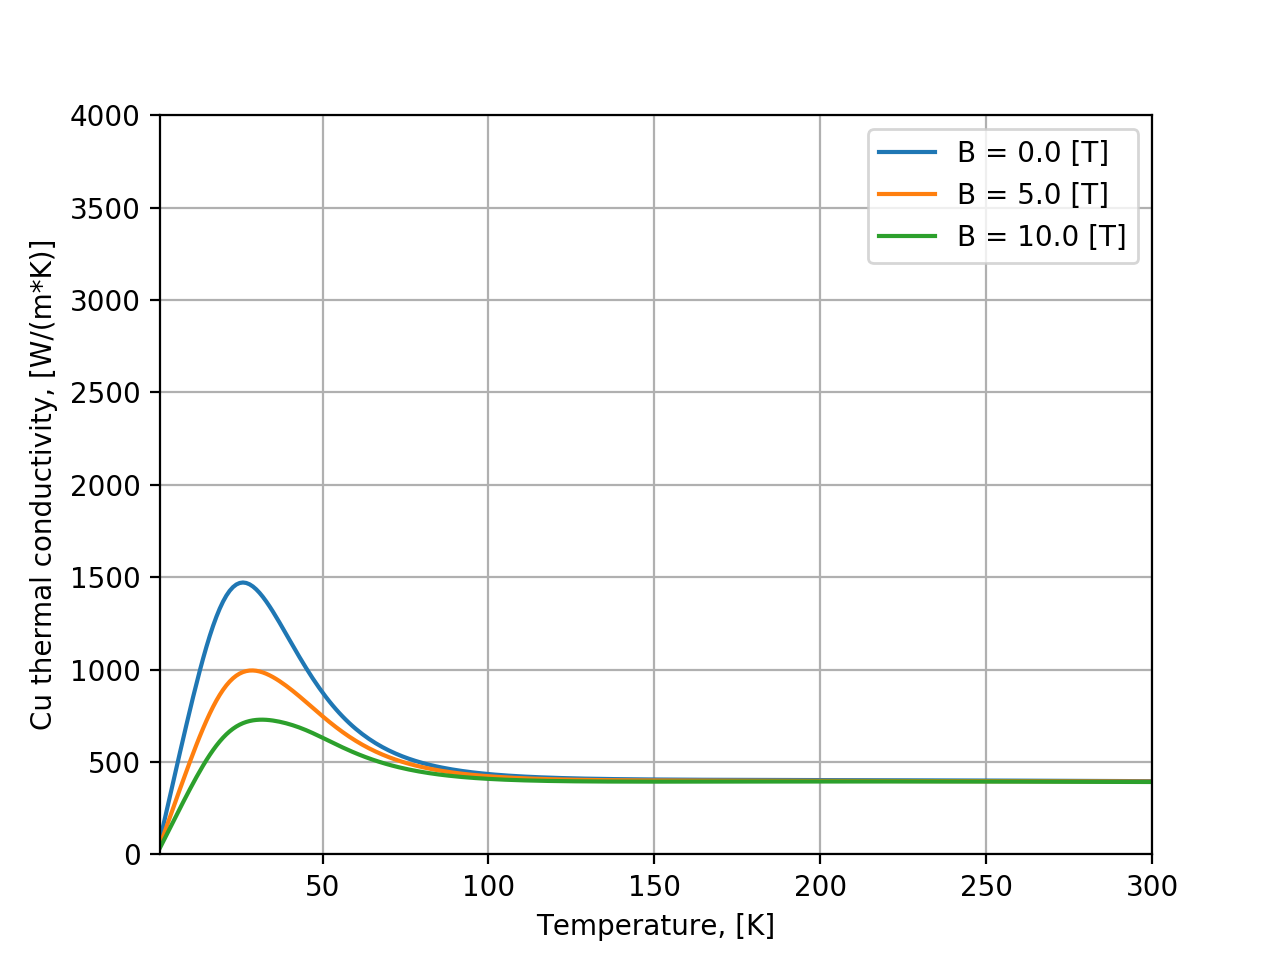
\includegraphics[width=0.49\linewidth]{figures/material_properties/Cu_k_B_Depenedence_plot_rrr_50.png}
    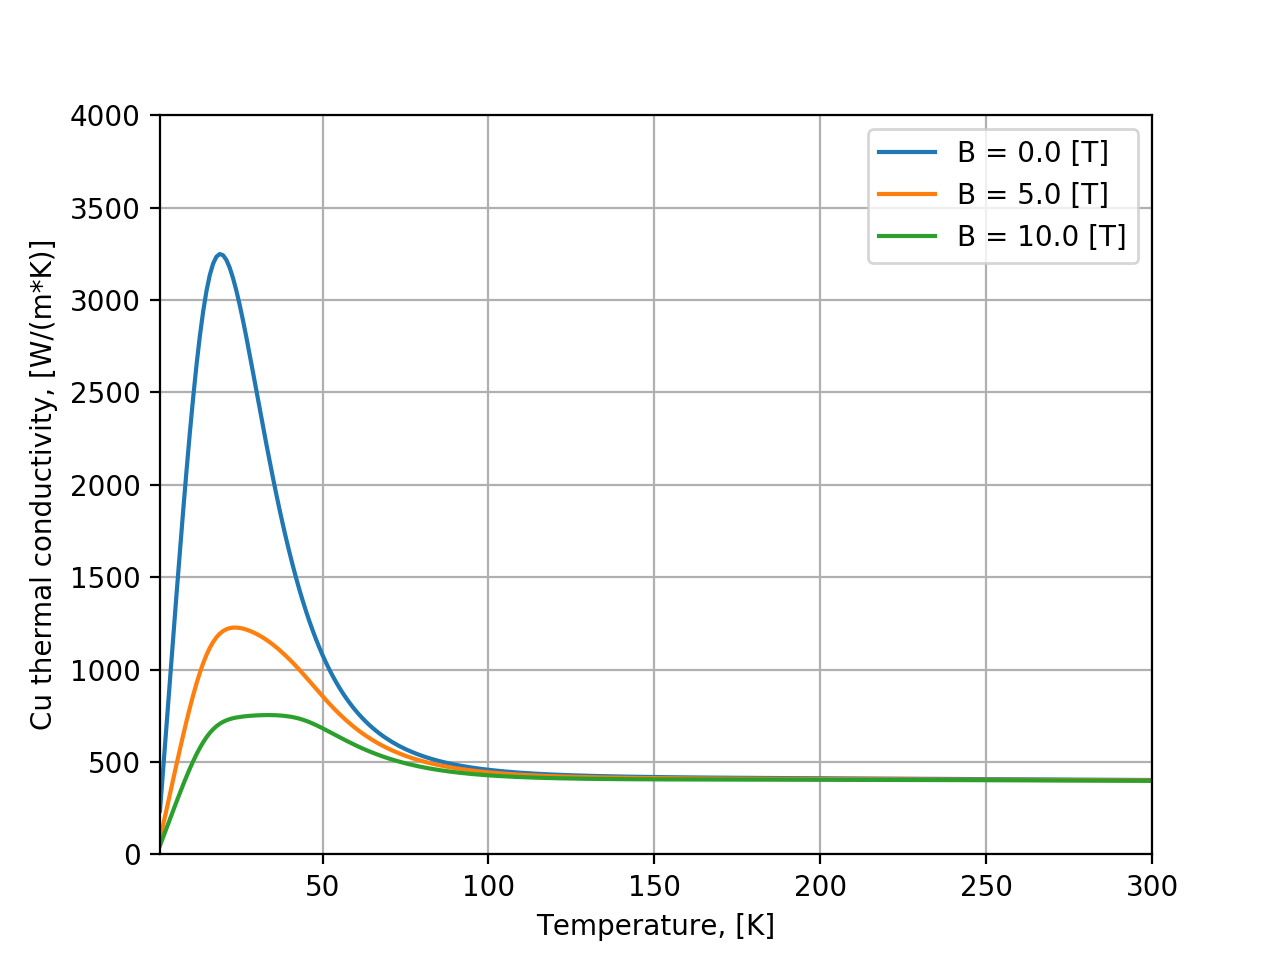
\includegraphics[width=0.49\linewidth]{figures/material_properties/Cu_k_B_Depenedence_plot_rrr_150.png}
    \caption{Copper thermal conductivity temperature dependence for three values of magnetic field for RRR = 50 (left) and RRR = 150 (right) }
    \label{fig:cu_k_plot}
\end{figure}

% mass density 
\subsubsection{Mass Density}
The mass density of copper is assumed to be constant and equal to $\rho = 8960~\text{kg/m}^{3}$.

% specific heat capacity 
\subsubsection{Specific Heat Capacity}
Copper specific heat capacity is approximated with the NIST polynomial interpolation. The fit with parameters described in Table \ref{table:nist_cu_cp_parameters}, is valid in the range between 4 and 300 K. It is assumed that the fit is valid throughout the entire analysis of quench.

\begin{equation}
    x(T) = 10^{\sum_{n=0}^{N} a_\text{n}(\log_\text{10}T)^{n}},
\end{equation}
\\
where $N$ refers to the order of polynomial.

\begin{table}[h!]
    \caption{Fit parameters for NIST copper specific heat capacity} 
    \vspace{-1.em} 
    \fontsize{10}{10}
    \selectfont 
    \renewcommand{\arraystretch}{1.5}
    \begin{center}
    \begin{tabular}{ cccccccc }  
    $\text{a}_0$ & $\text{a}_1$ & $\text{a}_2$ & $\text{a}_3$ & $\text{a}_4$ & $\text{a}_5$ & $\text{a}_6$ & $\text{a}_7$ \\
    \hline
    -1.91844 & -0.15973 & 8.61013 & -18.996 & 21.9661 & -12.7328 & 3.54322 & -0.3797 \\
    \hline 
    \end{tabular}
    \end{center}  
     \label{table:nist_cu_cp_parameters} 
 \end{table}

\begin{figure}[h!]
    \centering
    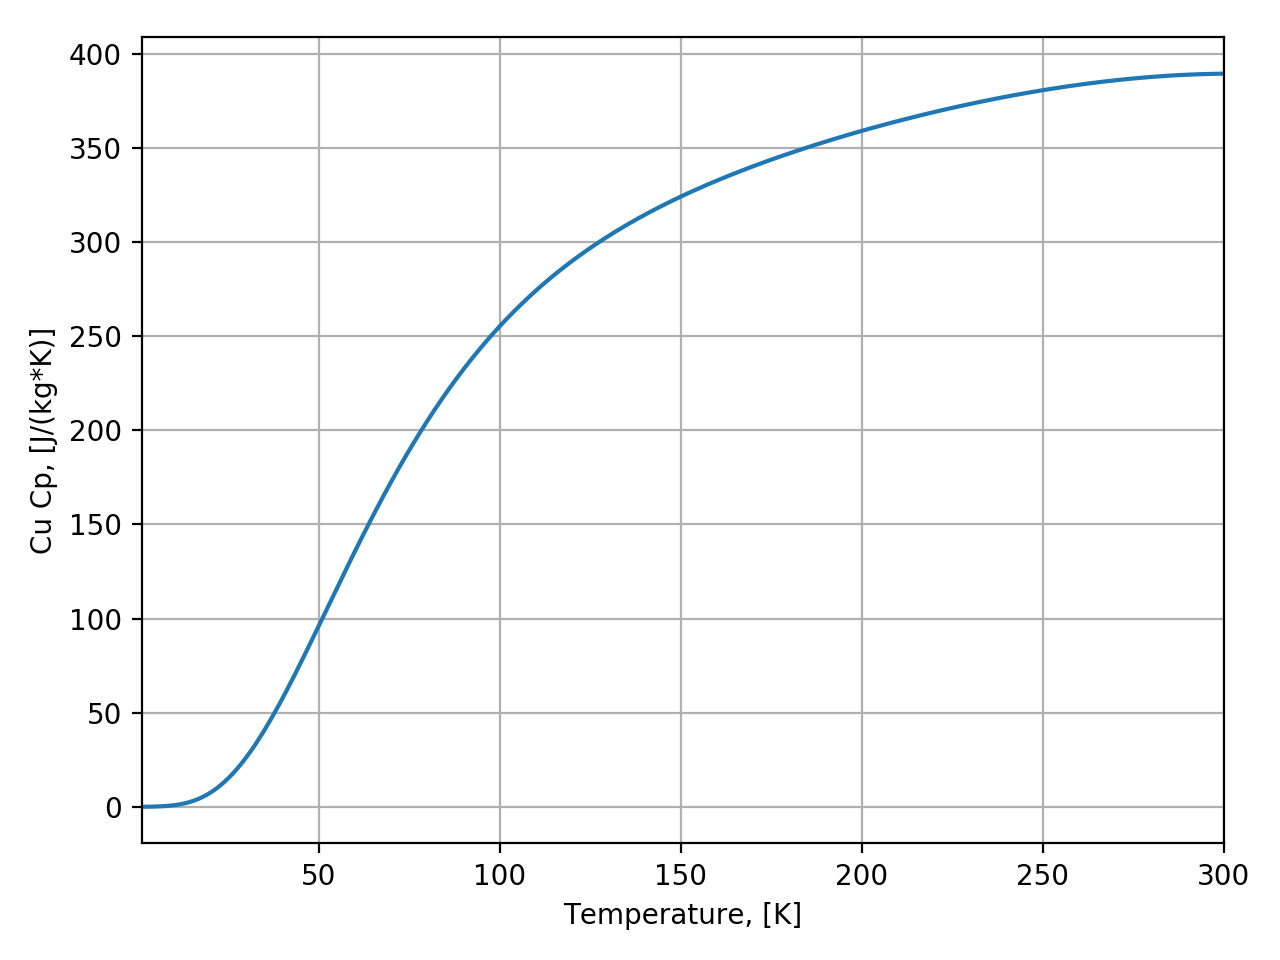
\includegraphics[width=0.49\linewidth]{figures/material_properties/Cu_Cp_plot.png}
    \caption{Copper specific heat capacity temperature dependence}
    \label{fig:cu_cp_plot}
\end{figure}
\newpage